\chapter{Introduction}
\label{sec:introduction}

\section{Motivation}
Information Retrieval systems become more important not only due to their use in Internet and digital libraries, but also because the majority of companies ( business ?) organize their activities and depend on digital documents, and information. Finding the right information brings value to the business, and failing to do so often leads to losses.\\

The search applications nowadays, whether used in Internet or in companies  internally, face constantly growing problem of information overload. Users searching for information usually submit queries composed of a few keywords only. The search application performs exact matching between the submitted keywords, and the document set it searches through, and often returns a long list of results. Users without domain expertise are not familiar with the appropriate terminology thus not submitting the right query terms with respect to relevance or specialization. Thus, users retrieve a large number of irrelevant pages. \\

\gls{IR} systems are facing challenges due to the peculiarities of human behavior, information overload, and information need.
\begin{itemize}
\item \textbf{Human behavior}. Users searching for information usually submit queries composed of a few keywords only, as shown in studies\cite{98usersSearchBehavior}. The search application performs exact matching between the submitted keywords, and the document set it searches through, and often returns a long list of results. When searching with short queries, the focus of a user is unclear, the missing information contributes to long result lists containing many unrelevant hits. Users without domain expertise are not familiar with the appropriate terminology thus not submitting the right query terms with respect to relevance or specialization. Another issue is the ambiguity of words, when words have more than one meaning. As a consequence, search results do not fit the information needs of users. When relevant documents contain words that are semantically relevant to the queries but not the same (synonyms), they will not be judged relevant. 
\item \textbf{Manual processing of results}. When a large number of matching documents is returned as a search result, only some of the documents found can be read, due to human limitations in information processing, and time constraints (users want to find information quickly). Human users need to narrow down the search iteratively by reformulating the query, since it is unclear in which context their queried words are used, and which words could be useful to focus the search. This reformulation is known as a frustrating and time consuming process.
\item \textbf{Information need}. Search applications that implement the keyword search paradigm (or full-text search) are broadly accepted by users; however, the challenge for the next years is the development of search solutions that reflect users' context ("what the user meant" versus "what the user wrote"). In other words, solutions that are able to:   
\begin{inparaenum}[\itshape a\upshape)]
\item  organize search results better than in the form of long lists,  
\item  adapt to a user�s personal skills and experience concerning the underlying document collection, and  
\item  adapt to the retrieval task a user is concerned with, 
\end{inparaenum}
or to adapt to the users' information need. \\
\end{itemize}


The issues listed above have lead to the development of techniques to assist users effectively navigate and organize the available documents in the search results, with the goal to find the best matching their needs. $Document clustering$ is a technique that offers methods to structure the search results in categories, in order to aid users in finding the best results for their search needs. It solves the problem of finding a meaningful ordering in a large amount of returned results.\\


When a categorization according to topic is determined using an unsupervised approach (document clustering), it has to be presented to the users. In particular, the categories have to be labeled with characteristic terms for browsing. Which words from the cluster to choose as labels is a difficult problem to solve. This work offers an overview of the current algorithms for cluster labeling. It evaluates an interesting new method for cluster labeling, called Weighted Centroid Covering, proposed in \cite{Stein04topicidentification} and \cite{Stein07topicidentification}. It further makes a proposal for improving the quality of identified labels, by using external knowledge from a light-weight ontology. This work further presents the ontology, developed for this purpose.\\

Another important aspect of the problem is to find comprehensive and accurate descriptions (labels) for the clusters of semantically related documents. \\

Information retrieval systems become more and more important, and have their main application areas in Internet, libraries, and in the business companies. \\

\gls{IR} technologies find wide application - in search engines, for browsing or filtering document collections, for further processing a set of retrieved documents. Before retrieval the documents are indexed, otherwise at each search, they would have to be scanned through for each query. The index maps the words or terms back to the documents where they occur. A method for document indexing, which is applied in this work, is called \gls{LSA}. It indexes the document collection by representing it as a reduced matrix of words and documents. \gls{LSA} representation improves \gls{IR} performance with respect to a basic problem of word-matching search - synonymy, or the case when more than one term describe the same concept. \\


\section{Information Retrieval systems}
In this work we investigate techniques from the field of \gls{IR}. Therefore, what follows is an overview of the text analysis processes, common to most \gls{IR} systems. Then, in the context of these processes, we shall summarize the contributions of the current work.\\

Most IR systems share common workflow, and follow common data processing stages.
The main goal of text analysis is knowledge discovery. There are many challenges today in the fields where text analysis is applied, and the main one is that there exists a huge amount of information to process manually. 
Another challenge is the data ambiguity, synonyms, polysemy.
We shall call text collections of documents a text corpus (pl. corpora).
Data in such collections can be structured, e.g. data in database tables, semi-structured, e.g. in XML, HTML format, or unstructured - articles, reports, e-mail, etc. \\

Text analysis processes involve information retrieval, lexical analysis to study word frequency distributions, tagging/annotation, among the others.\\

Automated processing, modeling, and analysis of unstruc-
tured text (news documents, web content, journal articles,
etc.) is a key task in many data analysis and decision mak-
ing applications. In many cases, documents are modeled as
term or feature vectors and latent semantic analysis (LSA)
[4] is used to model latent, or hidden, relationships between
documents and terms appearing in those documents. LSA
supplies conceptual organization and analysis of document
collections by modeling high-dimension feature vectors in
many fewer dimensions.



%
% text analysis sequence
%
\begin{figure}[htbp]
\label{fig:text_analysis}
	\centering
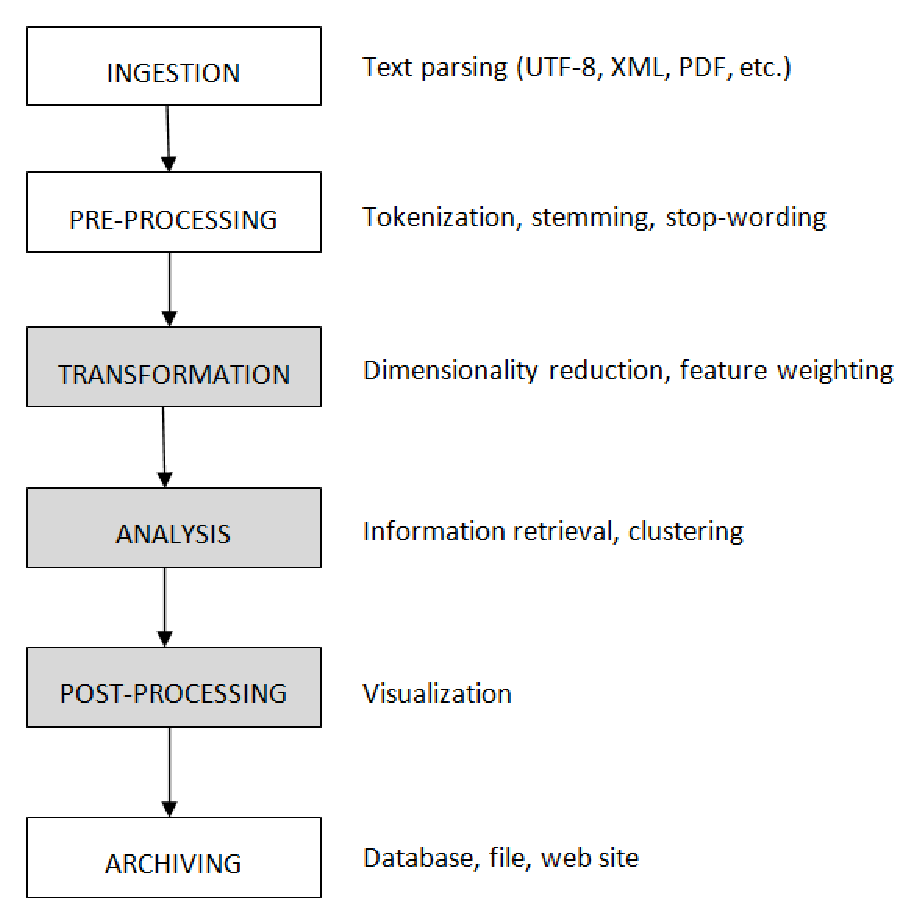
\includegraphics[width=\ScaleIfNeeded]{img/text_analysis}
%	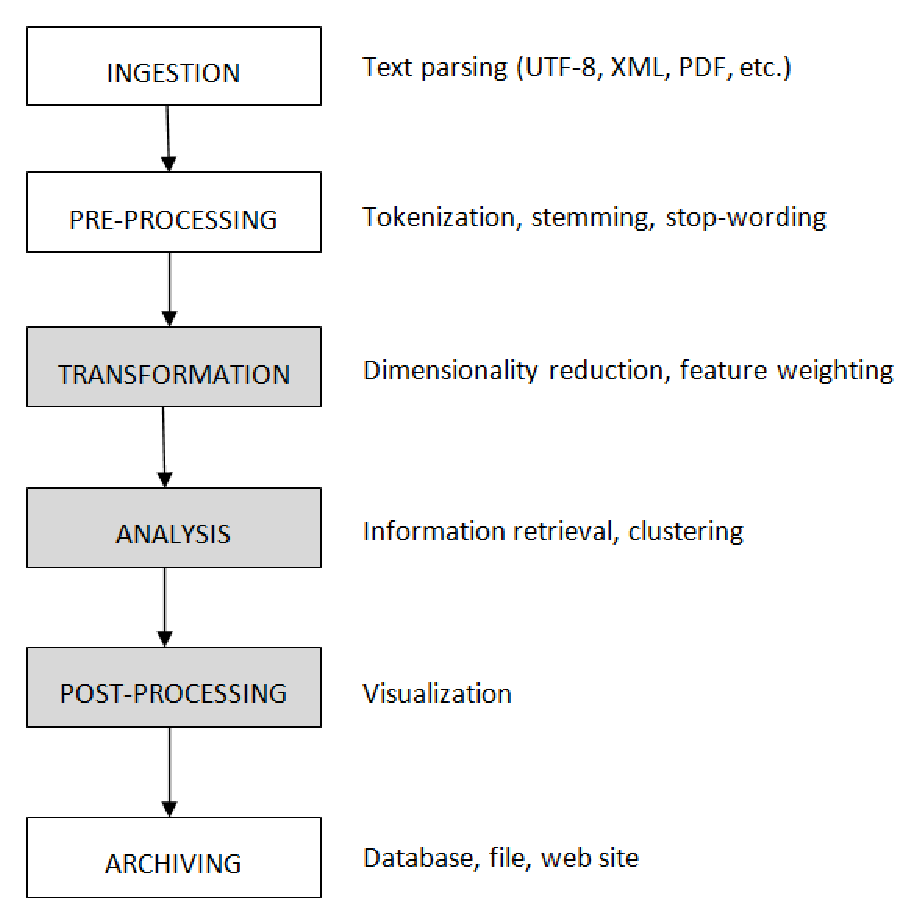
\includegraphics[width=\ScaleIfNeeded]{img/text_analysis} 
%\includegraphics[height = 0.7\textheight, trim = 30 100 30 280, clip, angle = 270]{timer}
 % or [scale=0.5]
	\caption[Workflow in IR systems]%
           {[Workflow in IR systems}
\end{figure}

The current work contributes in the transformation, analysis and post-processing phases of \gls{IR} workflow. The research focus is automatic identification of the main topics in a set of documents, returned as results to user queries. Research is done in analysis and visualization phases of the text analysis sequence diagram\ref{fig:text_analysis}. \\


This thesis contributes right here; techniques are developed which address the
design and the operationalization of IR processes respecting the above points.
The research focus is automatic document categorization, a technique which has
been shown to improve retrieval performance.\\


\section{Goal and scope of work}
This works contributes with the following:
\begin{enumerate}
\item It offers an overview of the current cluster labeling algorithms, and makes an evaluation of \gls{WCC}, proposed for unsupervised topic labeling of clusters in \cite{Stein04topicidentification} and \cite{Stein07topicidentification}.
\item It proposes an improvement in \gls{WCC} algorithm, performing topic identification based on external knowledge. A light-weight ontology has been developed for this purpose, in order to be used as a reference for external semantic knowledge during cluster labeling. 
\item A software application for executing an IR process has been developed. It implements \gls{LSA} for information retrieval, and \gls{WCC} for visualization of the main concepts contained in a document set in the form of a tag cloud. \\
\end{enumerate}


\section{Outline}
This chapter motivates the presented research work, and summarizes its contributions. It also offers a general overview to the phases of text analysis, common to most IR systems. Chapter 2 gives theoretical foundations for preprocessing and transformation phases of text analysis, and reviews a specific technique for information retrieval, called Latent Semantic Analysis. Chapter 3 contains the contribution related to evaluation of \gls{WCC} algorithm, and a proposal for its improvement, by using a light-weight ontology developed for this purpose. It represents the analytical phase in \gls{IR} systems. Chapter 4 refers to the post-processing phase of text analysis, giving the visualization means for presenting the main concepts retrieved from a document set. The software contribution, developed as a part of this work, is described in Chapter 5. Finally, in Chapter 6 the thesis concludes with evaluation of results and outlook.\\

